\documentclass[a4paper,parskip,11pt, DIV12]{scrreprt}

\usepackage[ngerman]{babel} % F��r Deutsch [english] zu [ngerman] �ndern. 
\usepackage[utf8]{inputenc}
\usepackage[T1]{fontenc}
\usepackage{blindtext}
\usepackage{graphicx}
\usepackage{subfigure}
\renewcommand{\familydefault}{\sfdefault}
\usepackage{helvet}
\usepackage{fancyhdr}
\usepackage{amsmath}
\usepackage{mdwlist} %Ben�tigt f��r Abst�nde in Aufz�hlungen zu l�schen
\usepackage{here}
\usepackage{calc}
\usepackage{hhline}
\usepackage{marginnote}
\usepackage{chngcntr}
\usepackage{tabularx}
\usepackage{titlesec} % Text��berschriften anpassen

% \titleformat{�berschriftenklasse}[Absatzformatierung]{Textformatierung} {Nummerierung}{Abstand zwischen Nummerierung und �berschriftentext}{Code vor der �berschrift}[Code nach der �berschrift]

% \titlespacing{�berschriftenklasse}{Linker Einzug}{Platz oberhalb}{Platz unterhalb}[rechter Einzug]

\titleformat{\chapter}{\LARGE\bfseries}{\thechapter\quad}{0pt}{}
\titleformat{\section}{\Large\bfseries}{\thesection\quad}{0pt}{}
\titleformat{\subsection}{\large\bfseries}{\thesubsection\quad}{0pt}{}
\titleformat{\subsubsection}{\normalsize\bfseries}{\thesubsubsection\quad}{0pt}{}

\titlespacing{\chapter}{0pt}{-2em}{6pt}
\titlespacing{\section}{0pt}{6pt}{-0.2em}
\titlespacing{\subsection}{0pt}{5pt}{-0.4em}
\titlespacing{\subsubsection}{0pt}{-0.3em}{-1em}

%\usepackage[singlespacing]{setspace}
%\usepackage[onehalfspacing]{setspace}

\usepackage[
			%includemp,				%marginalien in Textk�rper einbeziehen
			%includeall,
			%showframe,				%zeigt rahmen zum debuggen		
			marginparwidth=25mm, 	%breite der marginalien
			marginparsep=5mm,		%abstand marginalien - text
			reversemarginpar,		%marginalien links statt rechts
			%left=50mm,				%abstand von Seitenraendern
%			top=25mm,				%
%			bottom=50mm,
			]{geometry}		

%Bibliographie- Einstellungen
\usepackage[babel,german=quotes]{csquotes}
\usepackage[
   backend=bibtex8, 
   natbib=true,
    style=numeric,
    sorting=none
]{biblatex}
\bibliography{Quelle}
%Fertig Bibliographie- Einstellungen

\usepackage{hyperref}

\begin{document}
\selectlanguage{ngerman}
\begin{titlepage}
\begin{figure}[h]
\hfill
\subfigure{
\includegraphics[scale=0.04]{uzh}}
\end{figure}
\vspace{1 cm}
\textbf{\begin{huge}Praktikumsbericht Festk�rperphysik
\end{huge}}\\
\noindent\rule{\textwidth}{1.1 pt} \\

\begin{Large}\textbf{Widerstandsmessung am Halbleiter}
\end{Large}\\ 
\normalsize 
\par
\begingroup
\leftskip 0 cm
\rightskip\leftskip
\textbf{Modul:}\\ PHY210 \\ \\
\textbf{Assistent:}\\ Kay Waltar \\ \\
\textbf{Studenten:}\\ Nora Salgo, Manuel Sommerhalder, Fabian St�ger\\ \\
\textbf{Datum des Versuchs:}\\ 16.06.2017 \\ \\
\par
\endgroup
\clearpage



\end{titlepage}


%Start Layout
\pagestyle{fancy}
\fancyhead{} 
\fancyhead[R]{\small \leftmark}
\fancyhead[C]{\textbf{Widerstandsmessung am Halbleiter} } 
\fancyhead[L]{
\includegraphics[height=2\baselineskip]{uzh}}

\fancyfoot{}
\fancyfoot[R]{\small \thepage}
\fancyfoot[L]{}
\fancyfoot[C]{}
\renewcommand{\footrulewidth}{0.4pt} 

\addtolength{\headheight}{2\baselineskip}
\addtolength{\headheight}{0.6pt}


\renewcommand{\headrulewidth}{0.6pt}
\renewcommand{\footrulewidth}{0.4pt}
\fancypagestyle{plain}{				% plain redefinieren, damit wirklich alle seiten im gleichen stil sind (ausser titlepage)
\pagestyle{fancy}}

\renewcommand{\chaptermark}[1]{ \markboth{#1}{} } %Das aktuelle Kapitel soll nicht Gross geschriben und Nummeriertwerden

\counterwithout{figure}{chapter}
\counterwithout{table}{chapter}
%Ende Layout

\tableofcontents

\chapter{Einleitung}

\section{Überlegungen zum Versuch}

\begin{figure}[H]
\centering
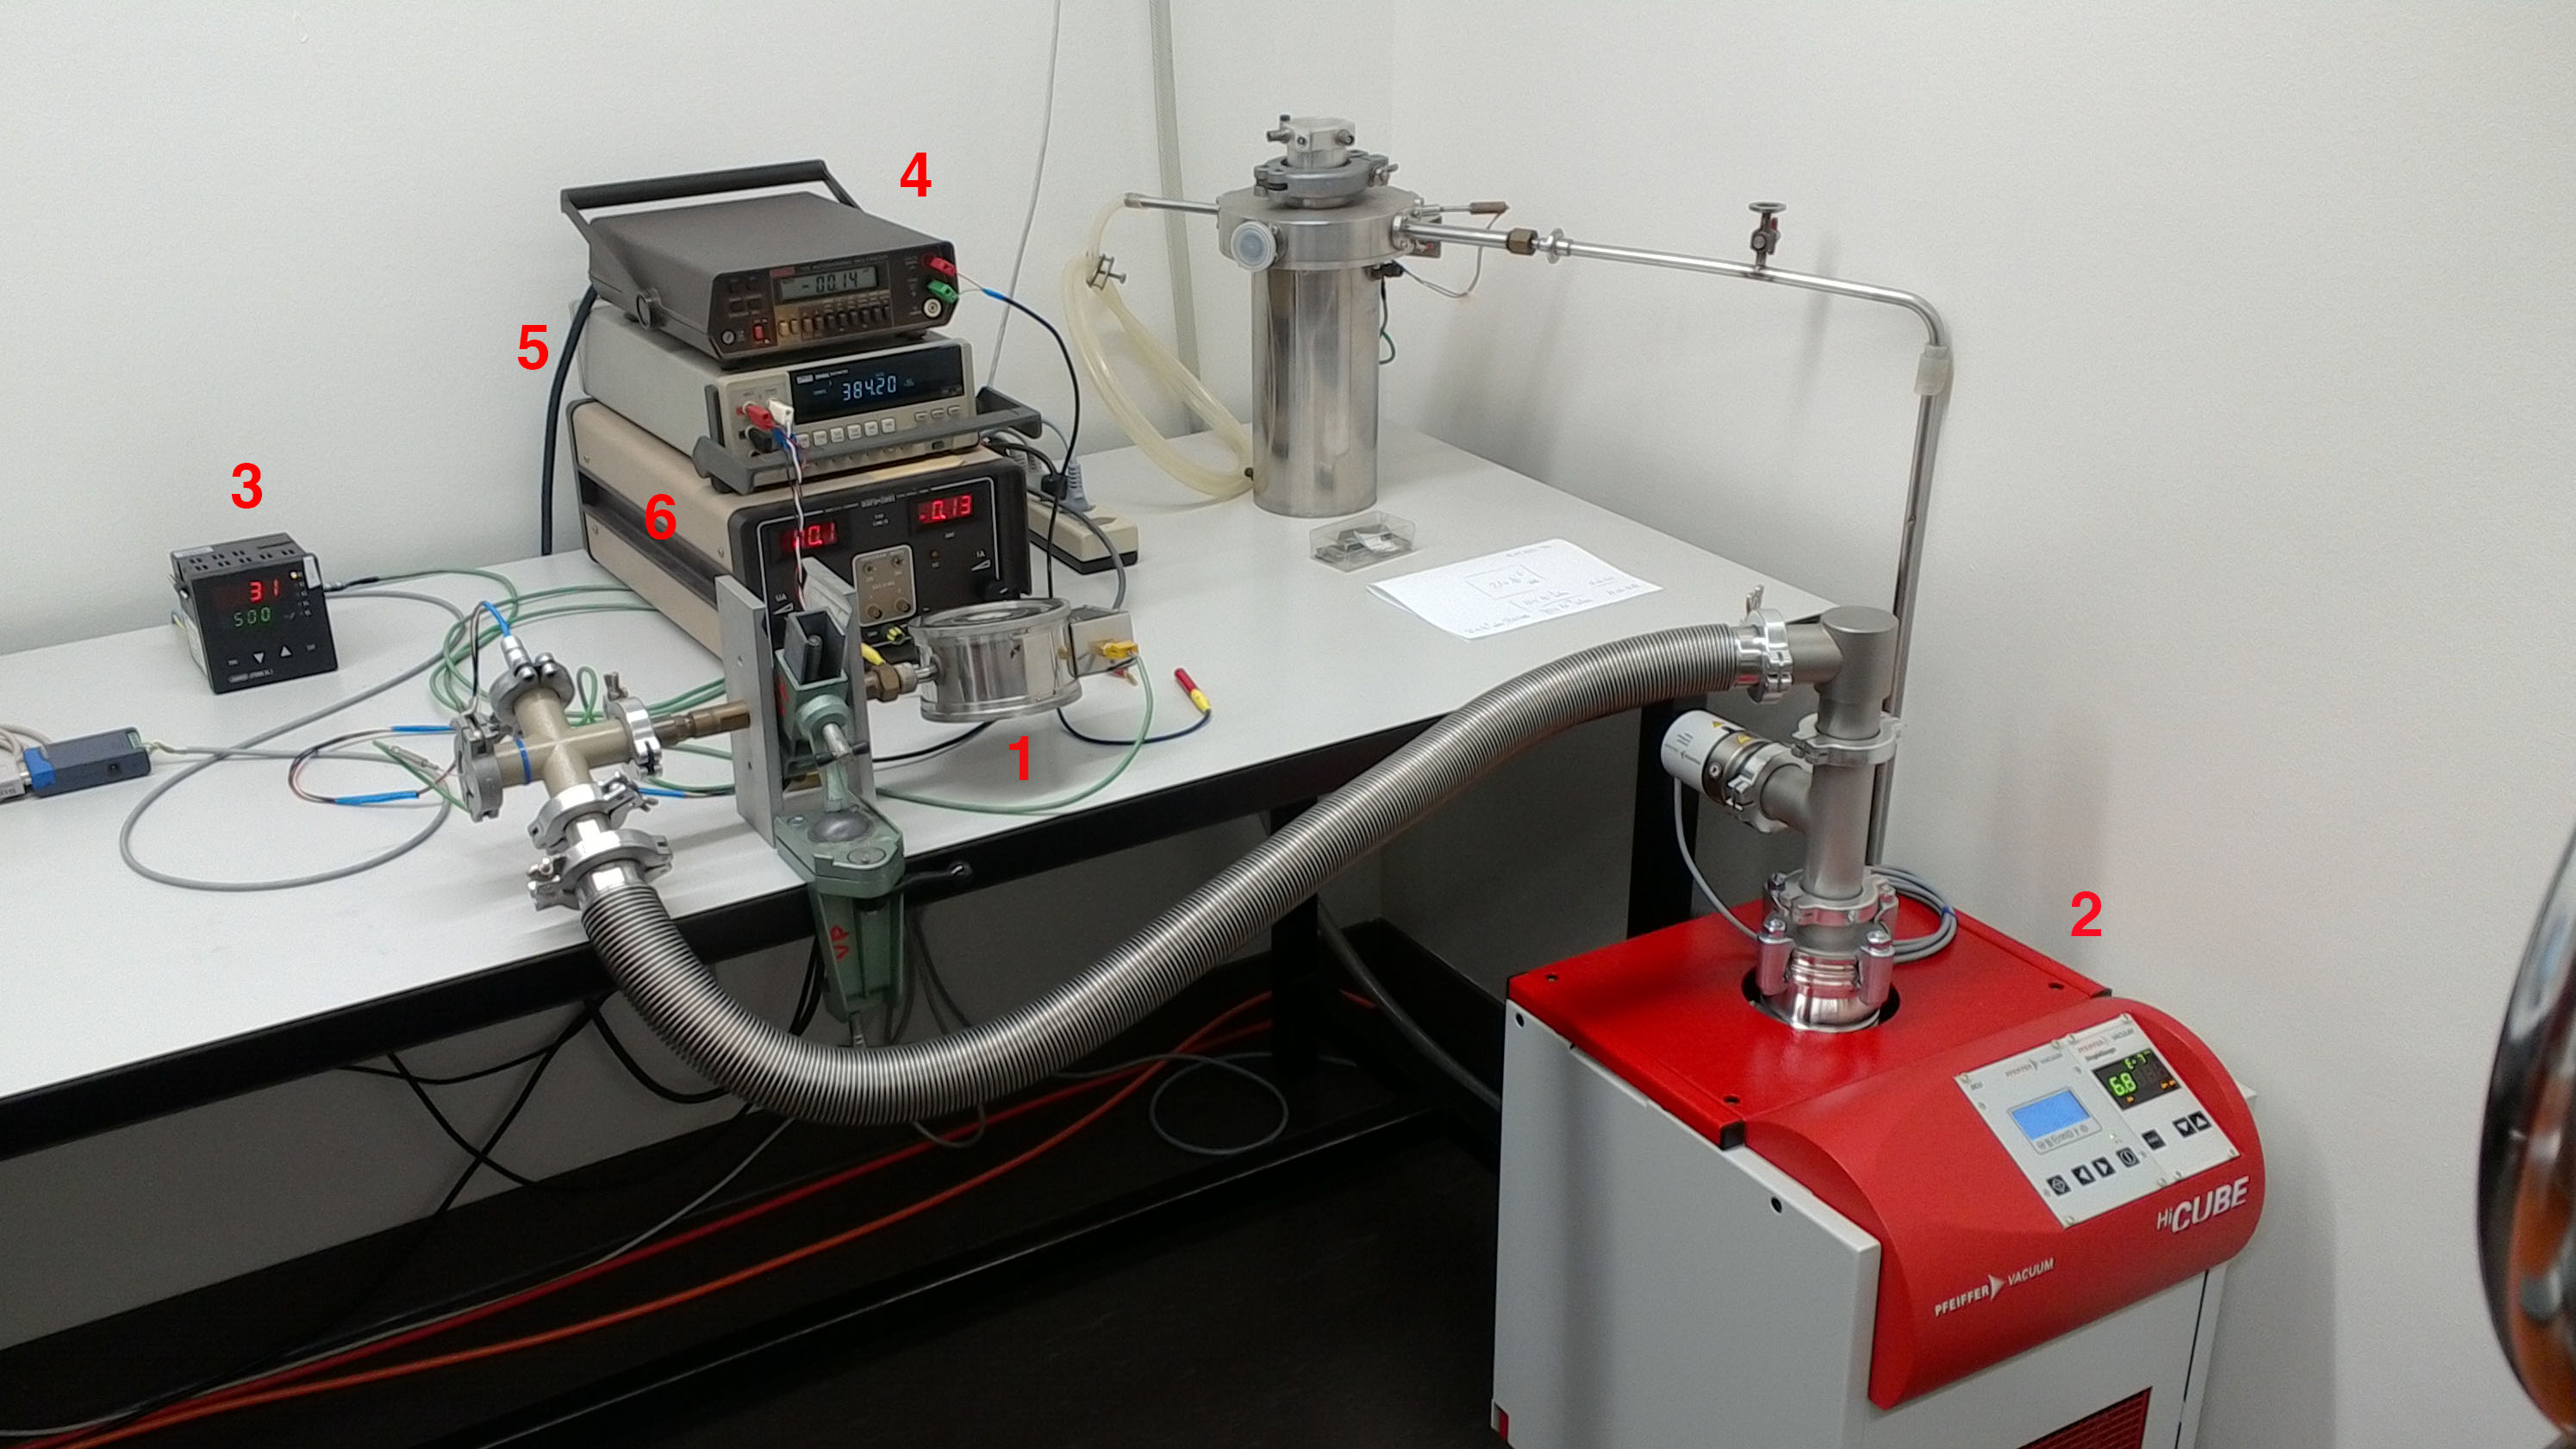
\includegraphics[keepaspectratio,width=\textwidth,height=\textheight]{Setup}
\caption[Setup]{Versuchsanordnung}
\label{Abb:Setup}
\end{figure}

\begin{equation} \label{Anleitungsformel}
u_e=\pm \frac{q}{3}=\frac{lL(1-\frac{L}{2l})m_{s,z} \frac{\partial B}{\partial z}}{6k_BT}
\end{equation}

\begin{align*}
&a_0 = 0.025459 \pm 0.002781 \quad
a_1 = 0.6113 \pm 0.0209 \\ 
&a_2 = 0.5146 \pm 0.0415 \quad
a_3 = -0.3907 \pm 0.0227
\end{align*} 

\begin{table}[H]
\centering
\renewcommand{\arraystretch}{1.2} % Abstandzwischen Zeilen
\setlength{\tabcolsep}{3mm} % Abstandzwischen Spalten
\begin{tabular}{|c|c|c|c|} 
$I$ [mA] & 			$B$ [T] & 					$T$ [K]  & 		$q$ [mm]\\ \hline
402   $\pm$ 5      & 0.306   $\pm$ 0.012   & 457.3  $\pm$ 0.1   & 2.2452 $\pm$ 0.0015 \\
600    $\pm$ 5      & 0.470   $\pm$ 0.021   & 459.5  $\pm$ 0.1   &3.5437  $\pm$ 0.0025\\
700    $\pm$ 5      & 0.549   $\pm$ 0.027  & 459.7   $\pm$ 0.1   &4.2096  $\pm$ 0.0029\\
800    $\pm$ 5     & 0.621    $\pm$ 0.034 & 459.7    $\pm$ 0.1   & 4.7810 $\pm$  0.0032 \\
900    $\pm$ 5     & 0.685    $\pm$ 0.042 & 459.9    $\pm$ 0.1    &5.3034  $\pm$  0.0032 \\
1000    $\pm$ 5    & 0.738     $\pm$ 0.052 & 460.7       $\pm$ 0.1 &5.7311  $\pm$ 0.0041
\end{tabular}
\caption[Daten]{Zusammenfassung der Daten}\label{tabelle1}
\end{table}

%\renewcommand{\bibname}{Quellenverzeichnis}
%\printbibliography

\end{document}
